\chapter{Background and Results from Preliminary Experiments}\label{sec:background}

This section gives brief background and results from preliminary experiments of the methods used to complete the Hubo-Ach system.
The motivation and timeline of experiments is given in Section~\ref{sec:roadmap}.

Section~\ref{sec:back:hubo-ach} describes why inter-process communication (IPC) is used for the Hubo-Ach control system and a brief background of different IPC methods.
Section~\ref{sec:hubo-ach} give this background in greater detail.


%%------ Path To Ph.D. -------%%	
	\section{Motivation}\label{sec:roadmap}	
		This section provides context to the origin of the idea of a unified algorithmic framework for complex systems.

%%%%%%% Put what I wrote here
\begin{figure}[thpb]
  \centering
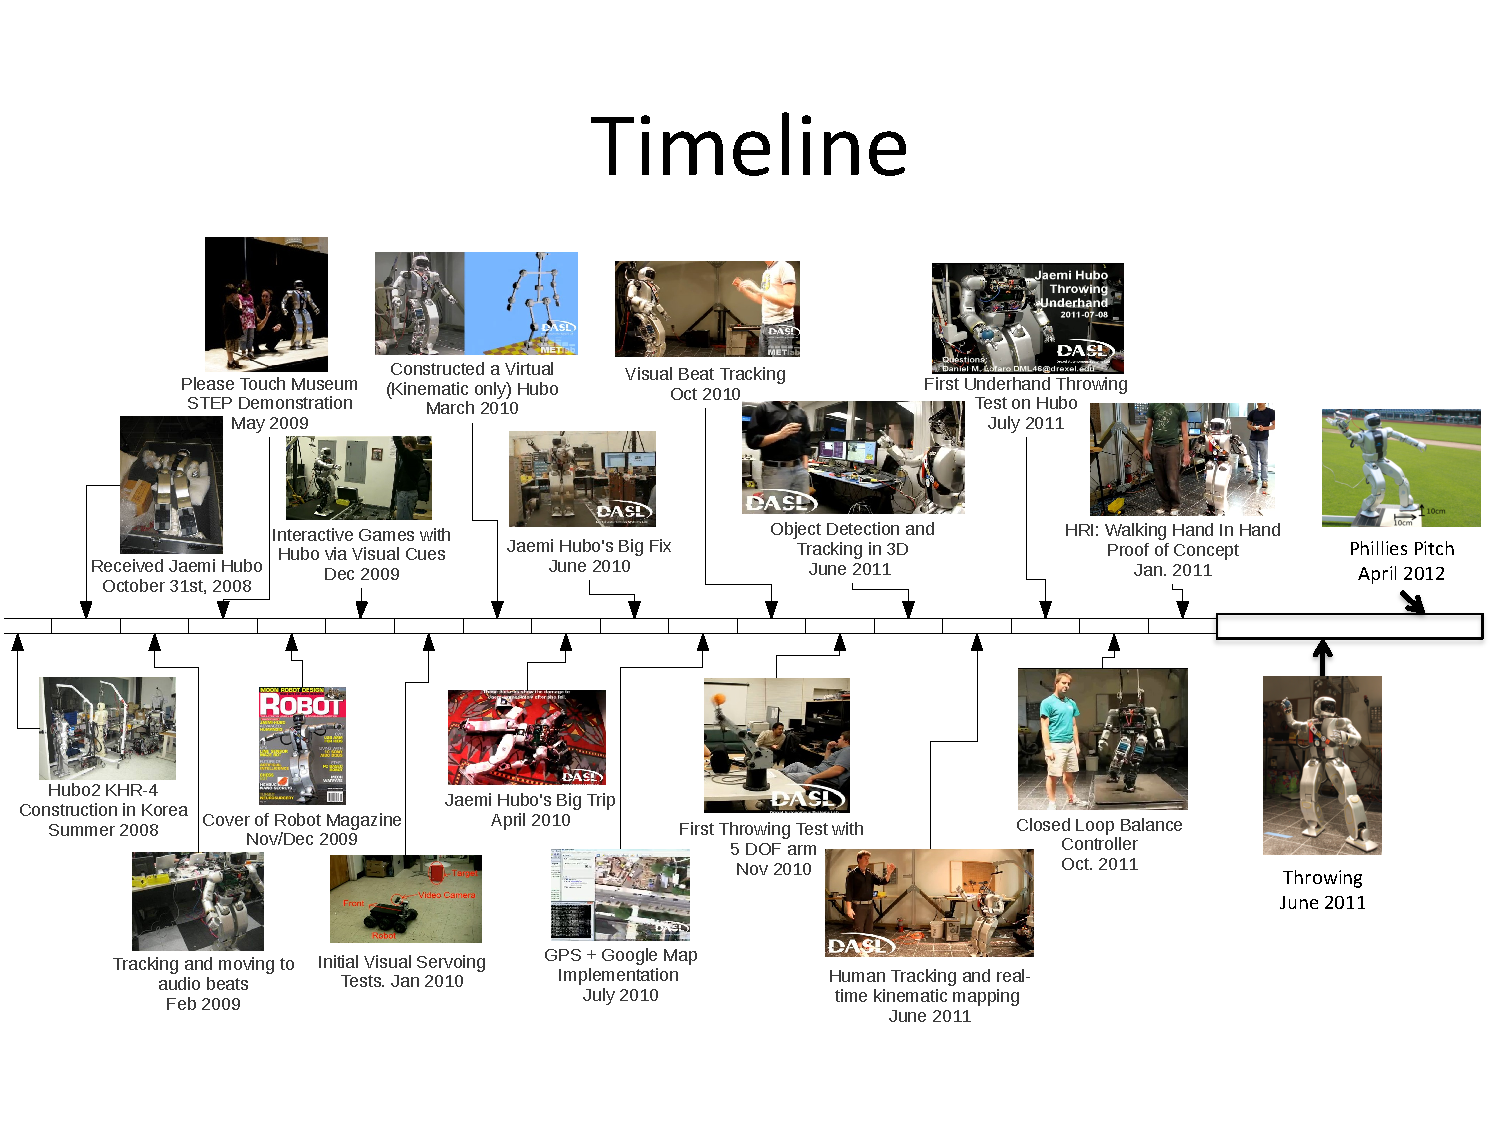
\includegraphics[angle=90, width=0.9\columnwidth]{./pix/Timeline.pdf}
  \caption{Timeline of Daniel M. Lofaro's research from 2008 to 2012}
  \label{fig:timeline}
\end{figure}

\subsection{Human Robot Interaction}
The initial goal was to have a humanoid robot become an interactive musical participant with humans.
This spawned the creation of a visual method of tracking the beat in the absence of auditory cues\cite{5686847}.
This came from a modification of a method of allowing children to play interactive games with humanoid robots\cite{lofaroGamesRobot}.
The resulting method was effective, but to increase the accuracy it was required to combine a pre-existing auditory beat tracker with the visual system.
This calumniated with a multi process system that combine the auditory and visual beat trackers\cite{lofaroIASTED2011,6094987,lofaroEURASIP2011}.
A human comparison was completed and found that this combined method was as accurate at detecting the beat in music as average humans.

\subsubsection{Results from preliminary experiments}
When collaborating with other to create a complex robot control systems integrating controllers is difficult because of the use of:
\begin{itemize}
\item different loop rates causing synchronization issues
\item different programming languages making using the same libraries a challenge
\end{itemize}

It was found that it is best to keep each working systems \textit{independent} allowing them to run at their native rate and on their native platforms\cite{ach}.



\subsection{High Degree of Freedom Kinematic Planning}
The next challenge was to perform kinematic planning for end effector velocity control. 
This resulted in the development of a method that is able to solve inverse kinematics (IK) for high degree of freedom (DOF) systems where there is no closed-form solution as well as create collision free trajectories for high DOF robots\cite{6385987}.
This is described in detail in Section~\ref{sec:srm} and \ref{sec:baseball}.
This culminated in the verification and validation of the system by an experiment where Hubo full-size humanoid robot throw the first pitch at a Major League Baseball (MLB) game\cite{lofaroHumanoids2012,6462956}.

\subsubsection{Results from preliminary experiments}
As best practice when controllers and planners are implemented it is important that low-level controllers such as balance and obstacle avoidance run at all times\cite{lofaroRAM2013}. 
Non-priority controllers such as throwing trajectory planning can run in the background in a separate process.
Keeping the processes separate allowed the system to be more resistant to lag and crashes of one or more of the controllers.
This brought validation to the overarching plan for the unified algorithmic framework for complex systems and humanoid robots.




\subsection{Lessons Learned}

At this point creating these experiment it was required to \textit{hacked} together pre-existing systems that allowed the robot to do the task.
This is the point where it was realized that a \textit{unified algorithmic framework for complex systems and humanoid robots} was required for further development in the field.
Key lessons learned from these experiments were:
\begin{itemize}
\item Must inherently decouple controllers loop rates and phases
\item Must allow for collaborators not have to \textit{inject} their code into existing source.
\item Must work with multiple robots for testing, evaluation, validation, and verification.
\end{itemize}

\noindent This is where Hubo-Ach was born.
The idea was to create a multi process architecture for humanoid control using state of the art high-speed low-latency Inter-Process Communication (IPC) techniques\cite{lofaroRAM2013}.
This is different from traditional IPC techniques because of the lack of head of line (HOL) blocking and focus on low-latency.
Section~\ref{sec:ipc} gives further details and comparisons of different IPCs.


The need for this unified framework was amplified when the Hubo was chosen to be the primary platform for the DRC-Hubo\footnote{DRC-Hubo: http://www.drc-hubo.com/} Track-A team.
Since its initial conception Hubo-Ach has become a fully functional system used in active research by multiple universities including MIT, WPI, Purdue, Ohio State, Swarthmore College, Georgia Tech, and Drexel University\cite{lofaroTePRA2013HuboAch,lofaroTePRA2013Valve}.
This research also acts as a key source of verification and validation of the system.


		

		\section{Control System Structures}\label{sec:back:struct}
			The traditional single loop control structure that is used in robot control software such as Orocos\cite{orocos-gadeyne-ijrr2005}, Microsoft Robot Studio\cite{microsoftRobot4437755}, RobotC\cite{robotc}, and LabVIEW\cite{labview} are not suited for high DOF robots.
Due to the nature of these highly redundant complex electrical mechanical system it is common to desire multiple different controllers running in tandem.  
Different controllers are needed when the system is in different states or doing different tasks or performing multiple tasks at the same time.
Combining these controllers is a problem in complex system.
This problem is hard when each controller has different loop rates that are not even multiples of on another, timing requirements (asynchronous vs. synchronous).

Multi-threaded approaches using shared memory allow for compatibility of multiple loop rates such as in Lee et. al.\cite{multi-thread-robot-5602743} with multi-threaded controllers on their humanoids, Rai et. al.\cite{multi-thread-snake-1541141} with multi-threaded controllers on their snake robots and Zheng et. al.\cite{multi-thread-5524083} with multi-threaded controllers on their under water robots.
The multi-threaded approach still has an inherent flaw.
If the parent or one of the other controller threads crashes it is difficult or impossible to restart the controller and still have access the the shared memory.

By using a multi process approach allows controllers to fault and restart with minimal effect on the other controllers.
Typical ways of communicating between different processes is via UDP or TCP/IP such as OpenHRP\cite{openHRP} with their server based control platform for the HRP humanoid robot; Aramaki et. al.\cite{multiPC-arch-1185243} and Lofaro et. al.\cite{lofaroIASTED2011} with their multi-computer based control methods and the popular Robot Operating System (ROS)\cite{ros} by Willow Garage.

Communicating via TCP/IP sockets, such as in OpenHRP and ROS, guarantee that the data is received but it does not guarantee a arrival time.
This means if the checksum fails the message will be sent again increasing the latency of the message.
This does not work well if a real-time control loop is required.
Using UDP does not resend if the checksum fails.
This keeps the latency low and is better for real-time applications such as in the work of Lofaro.
Both UDP and TCP/IP require that the buffer is read before new data is read.
This means that you must read the older data before newer data.
This is called head of line blocking or HOL\cite{ach}.

Newer state information is preferred by robots that work in the physical world over older data.  
Thus it is desired that HOL is eliminated.
This can be done with some forms of inter-process communication (IPC).

OpenHRP and Webots\cite{Webots} are two of the very short list of systems that have simulators that use the same controller as the hardware platforms.
However at this time to the best of our knowledge there is no system that:
\begin{itemize}
\item uses the same controller with the software and hardware systems
\item is inhreently robust by using a multi-process approach
\item uses low-latency methods for controller communications 
\end{itemize}





	
		\section{Multi-Process and Interprocess Comunication}\label{sec:back:hubo-ach}
	    		
This section gives a quick background to why inter-process communication (IPC) is used for the Hubo-Ach control system and a brief background of different IPC methods.
Section~\ref{sec:hubo-ach} give this background in greater detail.

The idea for a Control Architecture for High DOF robots stems from a gap in physical implementation of control algorithms for robot hardware.
The simplest approach to developing robot software is to integrate all functionality in one program.  
This functionality includes the following controllers:
\begin{multicols}{2}
\begin{itemize}
\item Hardware Control
\item Perception
\item Planning
\item Kinematics
\item etc.
\end{itemize}
\end{multicols}

If all of this functionality is in one process then it has the benefit of freedom of inter process communication latency.
However being in one process also means that if one of the controllers lags or faults it cause the entire controller to lag or fault.
This is of great concern if a non-priority controller such as vision processing faults causing a priority controller such as a balance controller, to fail.
This will cause the robot to fall.
How is this fixed?
One solution and my proposed solution is to use multiple processes and IPC methods.
Inter-process communication is a method of exchanging data between multiple processes.
Typical POSIX methods give you the \textbf{oldest} information first and have locks on the memory when processes are writing to it.
An overview of these mechanisms are given in \cite{stevens2005advanced}.

Robots work in the physical world. 
More recent information is more important to it then older.
In most cases it is acceptable to know the most recent data and never read any of the older data.
This would happen if your sensors update at a faster rate then that of the robot.
Typically robot actuators have a bandwidth much much lower then that of a modern computer.
If sensor information is shared using traditional shared memory over POSIX methods the controller would have to read the older information before it reaches the information it is most interested in, the newest data.
This is known effect but new concern for robot controllers called head of line blocking\cite{ach}.

It is desired to make a multi-process controller that can share data between multiple processes with low-latency and no head of line blocking.
There are a few IPCs that offer no head of line blocking and low-latency.  
A description of each IPC type is in Section~\ref{sec:hubo-ach}.
Table~\ref{table:ipc} shows a full comparison of the different IPC types.
%After much research (inserte examples here) it was found that the Ach IPC wuld best fit my needs.

My thesis Hubo-Ach is a multi-process control system that uses IPC methods to communicate between processes.
Section~\ref{sec:hubo-ach} describes Hubo-Ach in detail.



	    		
	    		
	%%------ About Hubo -------%%
	\section{Platforms}\label{sec:robots}
	This section describes the different platforms that are focused on in this document.
		\subsection{Hubo2 Plus}\label{sec:hubo}
			%\subsubsection{Hubo2 Plus}
The Hubo2+ is a $1.3\meter$ (4' 3'') tall, 42 $kg$ (93 $lb$) full-size
humanoid robot.  The Hubo series was designed and constructed by the
Korean Advanced Institute of Science and Technology (KAIST) and
spinoff Rainbow Inc. \cite{hubofirst}.  It has 38 degree of freedom:
six per arm and leg, five per hand, three in the neck, and one in the
waist.  Sensors include three-axis force-torque sensors in the wrists
and ankles, accelerometers in the feet, and an inertial measurement
unit (IMU).  The sensors and embedded motor controllers are connected
via a Controller Area Network to a pair of Intel Atom PC104+ PCs
running a GNU/Linux distribution.



% The reference commands for
% all of the joints are sent from the primary control computer (x86) to
% the individual motor controllers via two Controller Area Network (CAN)
% buses.  This is the same communications bus found in most modern motor
% vehicles.  There are currently eight Hubo's functioning in the United
% States as of December 2012.  Four reside at Drexel University and one
% at Georgia Tech, Purdue, Ohio State and MIT.  Jaemi Hubo is the oldest
% of the Hubos in America and has been at the Drexel Autonomous Systems
% Lab\footnote{Drexel Autonomous Systems Lab:
%   http://dasl.mem.drexel.edu/} (DASL) since 2008 \cite{jaemiHuboSRM}.
% Fig.~\ref{fig:hubo} shows the major dimensions of Hubo.

% \begin{figure}[thpb]
%   \centering
% \includegraphics[width=1.0\columnwidth]{./pix/huboSkel.pdf}
%   \caption{Hubo2 Plus platform: 38 DOF, 130 $cm$ tall full-size humanoid robot weighing 37 $kg$.}
%   \label{fig:hubo}
% \end{figure}

% All joints of the major joints are high gain PID position
% controlled with the exception of the fingers.  The fingers are
% open-loop PWM controlled.
% The sensing capability consists of a three
% axis force-torque (FT) sensor on each leg between the end of the ankle
% and the foot as well as between the arm where it connects to the hand.
% Additionally it has an inertial measurement unit (IMU) at the center
% of mass and accelerometers on each foot.

%%% Local Variables:
%%% mode: latex
%%% TeX-master: "ach"
%%% End:

		\subsection{Mini-Hubo}\label{sec:mini-hubo}
			Mini-Hubo\cite{threeTier} is a miniture version of the Hubo platform discribe in Section~\ref{sec:hubo}.
It is used as the Test and Evaluation (T\&E) stage of the three tier infrastructure discribed in Section~\ref{sec:threeTier}.
Mini-Hubo is kinematically scaled to the Hubo platform.
The atrobutes of the Mini-Hubo system are in Table~\ref{table:huboMiniSensors}.
The robot is shown in Fig.~\ref{fig:mini-hubo}


\begin{table}
\centering
\caption{Mini-Hubo Platform Specifications}
\begin{tabular}{| l || l |}
\hline
Height      		& $46~cm$			\\
\hline
Weight			& $2.9~kg$			\\
\hline
DOF			& 22				\\
\hline
Joint Control Type	& PID Position			\\
\hline
Computer		& $1.6~Ghz$ Atom		\\
			& $2~Gb$ DDR2 RAM		\\
\hline
Operating System	& Debian Linux			\\
\hline
Battery			& $14.8V$ $3.2~Ah$ $30C$ LiPo	\\
\hline
Sensors			& 2x 3 Axis Force Torque	\\
\hline
Vision			& Monocular			\\
			& RGBD				\\
\hline
\end{tabular}
\label{table:huboMiniSensors}
\end{table}





\begin{figure}[thpb]
  \centering
\includegraphics[width=0.37\columnwidth]{./pix/mini-hubo.jpg}
  \caption{Mini-Hubo platform: 22 DOF, 46 $cm$ tall miniture-size humanoid robot weighing 2.9 $kg$.}
  \label{fig:mini-hubo}
\end{figure}

		\subsection{OpenHubo}\label{sec:openhubo}
			OpenHubo\cite{dlofaro-srm} is an open-source kinematic and dynamic simulator for the the Hubo2 and Hubo2+ series robots.
It was developed by the Drexel Autonomous Systems Lab and runs using the open-source robot simulation environment OpenRAVE\cite{diankovThesis}.
Fig.~\ref{fig:openhubo1} shows the OpenHubo model.
Table~\ref{table:huboOpenSensors} shows the spesifications of OpenHubo.


\begin{figure}[thpb]
  \centering
      \includegraphics[width=0.4\columnwidth]{./pix/hBody.png}\includegraphics[width=0.4\columnwidth]{./pix/hCol.png}
      
\caption{OpenHubo model of the Hubo2 humanoid robot developed by the Drexel Autonomous Systems Lab and runs using the open-source robot simulation environment OpenRAVE\cite{diankovThesis}.}
\label{fig:openhubo1}
\end{figure}


\begin{table}
\centering
\caption{OpenHubo Platform Specifications}
\begin{tabular}{| l || l |}
\hline
Dynamics      		& Yes (ODE)			\\
\hline
Kinematic		& Yes				\\
\hline
DOF			& 40				\\
\hline
Joint Control Type	& PID Position			\\
\hline
Computer		& $1.6~Ghz$ Atom		\\
			& $2~Gb$ DDR2 RAM		\\
\hline
Enviroment		& OpenRAVE\cite{diankovThesis}	\\

\hline
Sensors			& 1x 4 Axis IMU			\\
			& 4x 3 Axis Force Torque	\\
\hline
\hline
\end{tabular}
\label{table:huboOpenSensors}
\end{table}

		
